\documentclass[tikz]{standalone}

\usetikzlibrary{patterns,decorations.markings}

\tikzset{
    cross/.style={fill=white,path picture={\draw[black]
        (path picture bounding box.south east) -- (path picture bounding box.north west)
        (path picture bounding box.south west) -- (path picture bounding box.north east);}},
    dressed/.style={fill=white,postaction={pattern=north east lines}},
    momentum/.style={->,semithick,yshift=5pt,shorten >=5pt,shorten <=5pt},
    loop/.style 2 args={thick,decoration={markings,mark=at position {#1} with {\arrow{>},\node[anchor=\pgfdecoratedangle-90,font=\footnotesize] {$p_{#2}$};}},postaction={decorate}},
    label/.style={thin,gray,shorten <=-1.5ex}
}

\def\lrad{1}
\def\mrad{0.175*\lrad}
\def\srad{0.15*\lrad}

\begin{document}
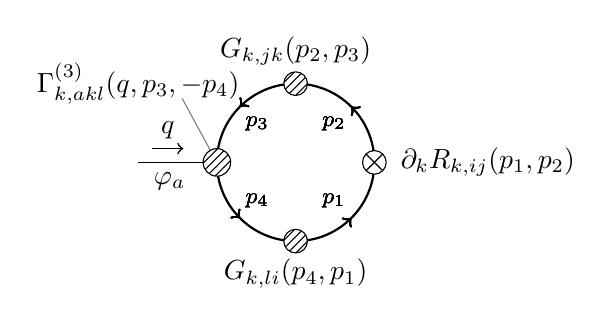
\begin{tikzpicture}[pin edge={shorten <=5*\lrad}]

  % Loop
  \draw[loop/.list={{0.125}{2},{0.125*3}{3},{0.125*5}{4},{0.125*7}{1}}] (0,0) circle (\lrad);
  \draw[cross] (\lrad,0) circle (\srad) node[right=6pt] {$\partial_k R_{k,ij}(p_1,p_2)$};
  \draw[dressed] (0,\lrad) circle (\srad) node[above=3pt] {$G_{k,jk}(p_2,p_3)$};
  \draw[dressed] (0,-\lrad) circle (\srad) node[below=3pt] {$G_{k,li}(p_4,p_1)$};

  % External line
  \draw (-2*\lrad,0) -- (-\lrad,0) node[pos=0.4,below] {$\varphi_a$};
  \draw[momentum] (-2*\lrad,0) -- (-1.25*\lrad,0) node[midway,above] {$q$};

  % Vertex
  \node (Gkakl) at (-2*\lrad,\lrad) {$\Gamma_{k,akl}^{(3)}(q,p_3,-p_4)$};
  \draw[label] (Gkakl.-30) -- (-\lrad,0);
  \draw[dressed] (-\lrad,0) circle (\mrad);

\end{tikzpicture}
\end{document}
